\chapter{Preliminaries}

\section{(Classical) Clustering}

First, let us define what a "clustering" is:
\begin{definition}
Let $(M, d)$ be a metric space, equipped with the metric function $d$.

\noindent Given a set of points $X \subset M$, a {\it $k$-clustering} of $X$ is a partition of $X$ into $k$ disjoint subsets, $C_1, \dots, C_k$, called {\it clusters}.
\end{definition}

An alternate formulation of definition would be to use something called an {\it assignment function}:

\begin{definition}
\begin{itemize}

\item A {\it $k$-clustering} of $X$ is an {\it assignment function}, $\alpha: X \rightarrow [k]$.

\item Each cluster $C_i$ is the preimage of $i$ under $\alpha$ i.e. $C_i = \alpha^{-1}(i)$

\end{itemize}
\end{definition}


There are many ways to quantify "how good a given clustering is". Depending on the objective, different variants of clustering problems are possible.
Here, we consider two specific types of $k$-clustering:

\begin{problem}[$k$-center problem]
Given a set of points $X \subset M$, find a $k$-clustering of $X$, denoted as $\mathcal{C}$, that minimizes
$$\phi(X, \mathcal{C}) = \max_{C \in \mathcal{C}} \left[ \min_{c \in C} \max_{x \in C} d(x, c) \right]$$
\end{problem}

\begin{problem}[$k$-median problem]
Given a set of points $X \subset M$, find a $k$-clustering of $X$, denoted as $\mathcal{C}$, that minimizes
$$\psi(X, \mathcal{C}) = \sum_{C \in \mathcal{C}} \left[ \min_{c \in C} \sum_{x \in C} d(x, c) \right]$$
\end{problem}


\section{Incorporating Fairness}

Now we ask ourselves how to incorporate fairness into above problems.
To consider a "fair" version of clustering, we first have to identify the {\it unprotected attribute} and {\it protected attribute}.
We shall consider the {\it coordinate} as the unprotected attribute. For simplicity, let us represent the protected attribute as the {\it coloring} of the points.
To simplify things further (as in the paper), let us only consider the case of binary coloring.


For $Y \subset X$, let us denote:
\begin{itemize}
	\item $\chi : X \rightarrow \{\text{RED}, \text{BLUE}\}$ is the given binary coloring.
	\item $R(Y) = \{x \in X : \chi(x) = \text{RED}\}$, $r(Y) = |R(Y)|$
	\item $B(Y) = \{x \in X : \chi(x) = \text{BLUE}\}$, $b(Y) = |B(Y)|$
\end{itemize}

\begin{definition}
\begin{itemize}
\item For $\emptyset \not= Y \subset X$, the {\it balance} of $Y$ is defined as:
$$\balance(Y) = \min \left( \frac{r(Y)}{b(Y)}, \frac{b(Y)}{r(Y)} \right) \in [0, 1]$$

\item The {\it balance} of a clustering $\mathcal{C}$ is defined as:
$$\balance(\mathcal{C}) = \min_{C \in \mathcal{C}} \balance(C)$$

\item If $\balance(Y)$ is $0$(resp. $1$), $Y$ is fully unbalanced(resp. perfectly balanced)
\end{itemize}
\end{definition}

Let's call a clustering algorithm {\it colorblind} if it doesn't take the protected attribute (coloring) into its decision making. It is easy to make an instance (and it is actually common) where colorblind algorithm results in a very unfair clustering. (Unfair in the sense that the resulting clustering is very unbalanced)
\begin{figure}[hbt!]
	\centering
	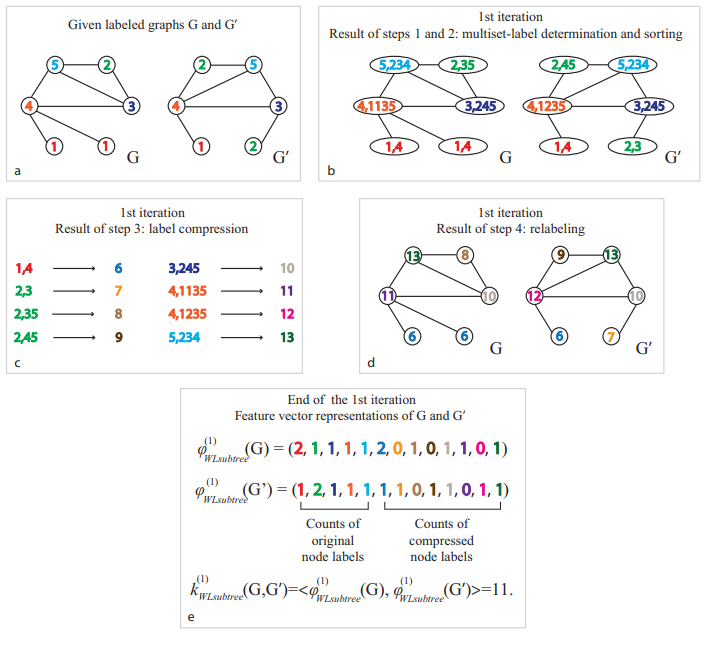
\includegraphics[height=3cm]{preliminaries/fig/fig1.png}
	\caption{An instance where a colorblind clustering produces an unfair result}
\end{figure}

{\it Therefore a "fair" clustering must take into account not just the position of the centers, but also the assignment function!}



\section{Fairlets and Fair Clustering}

\begin{definition}
Let $b, r$ be some integers such that $1 \leq b \leq r$ and $\gcd(b, r) = 1$.

\begin{itemize}
	\item A clustering $\mathcal{Y}$ of $X$ is called a {\it $(b, r)-$fairlet decomposition of $X$} if
	(i) $\forall Y \in \mathcal{Y} \ |Y| \leq b + r$ and (ii) $\balance(\mathcal{Y}) = b/r = \balance(X)$
	
	\item Each $Y \in \mathcal{Y}$ is called a {\it $(b, r)-$fairlet}, or simply {\it fairlet}.

\end{itemize}
\end{definition}

Intuitively, fairlet can be thought of as {\bf a group of points that are fair and cannot be split further into true subsets that are also fair}. Observe that the balance of the original set of points is preserved while keeping each cluster "small".

\begin{lemma}
Let $\balance(X) = b/r$ for some integers $1 \leq b \leq r$ such that $\gcd(b, r) = 1$.

\noindent Then there exists a $(b, r)-$fairlet decomposition of $X$.
\end{lemma}

This lemma tells us that every fair solution to the clustering problem induces a set of minimal fairlets, as shown in below figure:

\begin{figure}[hbt]
	\centering
	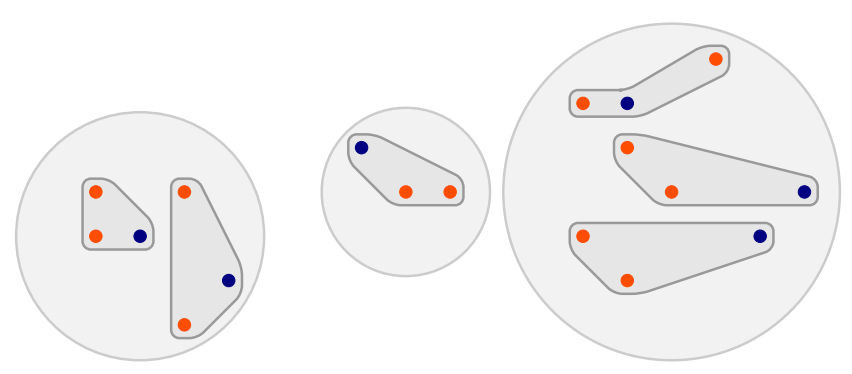
\includegraphics[height=2.6cm]{preliminaries/fig/fig2.png}
	\caption{A decomposition of a fair clustering into fairlets with two red points and one blue point}
\end{figure}

\newpage
Below is the final formulation of a "fair clustering":

\begin{problem}[$(t, k)-$fair center (resp. median) problem]
Partition $X$ into $\mathcal{C}$ such that
	\begin{itemize}
		\item $|\mathcal{C}| = k$
		\item $\balance(\mathcal{C}) \geq t$
		\item $\phi(X, \mathcal{C})$ (resp. $\psi(X, \mathcal{C})$) is minimized.
	\end{itemize}
\end{problem}

Note that if fairness is not taken into account ($t = 0$), the assignment function is implicit through a set $\{c_1, \dots, c_k\}$ of centers i.e.
	$$\alpha(x) = \argmin_{i \in [k]} d(x, c_i)$$
and thus equivalent with the classical clustering algorithm.
However with fairness taken into account, an explicit assignment function is required.
